\chapter{$\chi^2$ - Badanie jakości dopasowania śladów}
Krytycznym punktem każdego eksperymentu fizycznego jest, poza dokonanie niezbędnych pomiarów przeanalizowanie ich. Główne metody analizy danych doświadczalnych bazują na statystyce. W większości przypadków do zebranych danych eksperymentator stara się dopasować pewien model. Dopasowywany model powinien być tak dobrany, aby możliwe było wyznaczenie pewnych, poszukiwanych parametrów. 

Dlatego kluczowym elementem podczas przeprawiania analizy danych powinna być weryfikacja otrzymanych wyników. Niska jakość dopasania modelu do danych przekłada się na fakt, iż otrzymane wyniki są mało wiarygodne. Badanie jakości daje możliwość weryfikacji poprawności wyboru danego modelu. Głównym narzędziem służącym do tego jest test $\chi^2$.


\section{Definicja $\chi^2$}

Niech próbka zawiera $\nu$  niezależnych zmiennych $x_i$  pochodzących z rozkładów normalnych o średnich $\mu_i$ oraz wariancjach $\sigma_i$, to wielkość nazywana $\chi^2$ \footnote{Warto zwrócić uwagę, że używana nazwa $\chi^2$ może być myląca, gdyż jest to pojedyncza statystyczna zmienna a nie kwadrat jakiejś wielkości $\chi$. Notacja ta powinna być rozumiana w sensie, że wielkość ta składa się z sumy kwadratów.} jest definiowana jako

\begin{eqnarray}
\chi^2 &=& \frac{(x_1-\mu_1)^2}{\sigma_1^2}+\frac{(x_2-\mu_2)^2}{\sigma_2^2}+\ldots + \frac{(x_\nu-\mu_\nu)^2}{\sigma_\nu^2} \nonumber \\
&=& \sum_{i=0}^{\nu}\frac{(x_i-\mu_i)^2}{\sigma_i^2}
\label{chiRownanie}
\end{eqnarray}

W idealnym przypadku, po uwzględnieniu przypadkowych fluktuacji każdy z czynników sumy \ref{chiRownanie} powinien być rzędu jedności. Zatem przy założeniu dobrania odpowiednich wartości  $\mu_i$ oraz $\sigma_i$ powinno się spodziewać, że obliczona wartość $\chi^2$ powinna się zbliżać do $\nu$. Jeżeli tak jest, to uzasadnione jest wyciągnięcie wniosku, że dane opisane są dobrze przez wartości $\mu_i$ czyli innymi słowami hipotetyczną funkcję. 
Z drugiej strony, jeżeli wartość sumy $\chi^2$ znacznie odbiega od $\nu$ prawdopodobnie wybrany model nie opisuje zbyt dokładnie zmierzonych danych. 

Powyżej przedstawiono ogólną idee stojącą za testem $\chi^2$. W następnych częściach tego rozdziału omówione jak wygląda procedura przeprowadzania takiego testu.

\section{Rozkład $\chi^2$}

Wielkość  $\chi^2$ zdefiniowana równaniem \ref{chiRownanie} posiada funkcję gęstości prawdopodobieństwa daną równaniem: 

\begin{equation}
f(\chi^2)=\frac{1}{2^{0.5 \nu} \Gamma(\frac{\nu}{2})}e^{\frac{\nu^2}{2}} \left( \chi^2 \right)^{\frac{\nu^2}{2}-1}
\label{chi2Dis}
\end{equation}

Funkcja przedstawiona powyżej (równanie \ref{chiRownanie}) zwana jest rozkładem  $\chi^2$  o $\nu$ stopniach swobody, przy czym $\nu \in \mathbb{N}_{+}$. Na rysunku \ref{fig:chi2} zamieszczony 

\begin{figure}[h]
  \centering
  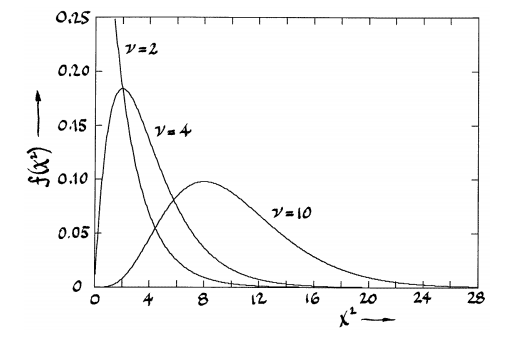
\includegraphics[scale=0.7]{rozdzial5/chi2.png}
  % AccComple.gif: 480x434 pixel, 72dpi, 16.93x15.31 cm, bb=0 0 480 434
  \caption{Funkcja rozkładu prawdopodobieństwa $\chi^2$  dla $\nu=2,4,10$.}
  \label{fig:chi2}
\end{figure}